%%%%%%%%%%%%%%%%%%%%%%%%%%%%%%%%%%%%%%%%%
% University/School Laboratory Report
% LaTeX Template
% Version 3.1 (25/3/14)
%
% This template has been downloaded from:
% http://www.LaTeXTemplates.com
%
% Original author:
% Linux and Unix Users Group at Virginia Tech Wiki 
% (https://vtluug.org/wiki/Example_LaTeX_chem_lab_report)
%
% License:
% CC BY-NC-SA 3.0 (http://creativecommons.org/licenses/by-nc-sa/3.0/)
%
%%%%%%%%%%%%%%%%%%%%%%%%%%%%%%%%%%%%%%%%%

%----------------------------------------------------------------------------------------
%	PACKAGES AND DOCUMENT CONFIGURATIONS
%----------------------------------------------------------------------------------------

%\documentclass{article}
\documentclass[a4paper,11pt]{exam}


\usepackage[version=3]{mhchem} % Package for chemical equation typesetting
\usepackage{siunitx} % Provides the \SI{}{} and \si{} command for typesetting SI units
\usepackage{graphicx} % Required for the inclusion of images
\usepackage{natbib} % Required to change bibliography style to APA
\usepackage{amsmath} % Required for some math elements 
\usepackage{float}
\usepackage{amsfonts}
\usepackage{bbold}
\usepackage{diagbox}
\usepackage{listings}


\printanswers
\setlength\parindent{0pt} % Removes all indentation from paragraphs

\renewcommand{\labelenumi}{\alph{enumi}.} % Make numbering in the enumerate environment by letter rather than number (e.g. section 6)

\usepackage{titlesec}


%\usepackage{times} % Uncomment to use the Times New Roman font

%----------------------------------------------------------------------------------------
%	DOCUMENT INFORMATION
%----------------------------------------------------------------------------------------

\title{Assignment 1: Instance-level recognition \\ Computer Vision Object Recognition} % Title
\author{Thomas \textsc{Opsomer}} % Author name

\date{\today} % Date for the report

\begin{document}

\maketitle % Insert the title, author and date


%----------------------------------------------------------------------------------------
%	Assignments 1
%----------------------------------------------------------------------------------------


%----------------------------------------------------------------------------------------
%	Part I
%----------------------------------------------------------------------------------------

\section{Sparse features for matching specific objects in images}

\subsection{SIFT features detections}

\textbf{QIA.1: Why is it important to obtain similarity co-variant features for matching?\\}

Given a picture of an object, and an other picture of the same object, we can find a transformation that turn the first point of view into the second one. This transformation is an homography. Homographies are group of transformation that contains particular subgroups: affine and similarity transformation. Similarity group is actually also a subgroup of affine transformations. So the simplest approximation of the transformation between the two points of view, is a similaritiy (of course it won't be the ideal one if the view changes are abrupt). Under this approximation, if we can obtain a representation of both images that is co-variant with translation, rotation and homothety (similarity transformation), then we can compare pictures based what are object are inside independently of the whole configuration of objects, points of view: angle, scale ...
\\

\textbf{QIA.2: Show the detected features in the two images for three different values of the peakThreshold\\}

\begin{figure}[!h]
\centering
\includegraphics[width=13cm]{figure/sift_threshold_impact.eps}
\caption{Compare SIFT features for thresholdPeak from 0.01 (left) to 0.0001 (right)}    
\label{sift_threshold_impact}
\end{figure}

\textbf{QIA.3: Note the change in density of detections across images. Why does it change? Which implications for image matching can this have? How can it be avoided?\\}

When comparing features extraction on the two images 1 and 2 (not the rotated one). We can see that the variation in density of detections is related to the brightness of the picture. More keypoints are found in the enlightened part of the building. This behavior can impact severely the task of image matching. Though the representation is co-variant with similarity transformation it seems to vary with the illumination of objects (shadow, light, enlightened parts...), consequently large variations in illumination conditions (light exposure ...) could affect the performance for matching.
\\
To avoid this effect we would need a feature that is invariant with illumination but SIFT doesn't do that. However we could preprocess images to normalize contrast and level equalization, which should improve SIFT feature detection in different illumination configuration but it won't solve the main problem, just reduce it.

\begin{figure}[!h]
\centering
\includegraphics[width=13cm]{figure/sift_im1_im2.eps}
\caption{Compare SIFT features on image1 and image2}    
\label{sift_im1_im2}
\end{figure}

\subsection{SIFT features descriptors and matching between images}

\textbf{QIB.1: Note the descriptors are computed over a much larger region (shown in blue) than the detection (shown in green). Why should this be a good strategy?\\}

\begin{figure}[!h]
\centering
\includegraphics[width=13cm]{figure/sift_descriptors.eps}
\caption{SIFT Descriptors}    
\label{sift_descriptors}
\end{figure}

SIFT Descritors are represented in figure \ref{sift_descriptors}.\\
Descriptors needs to describe distinctively the detectors and to be locally invariant as possible to any changes (rotation, illumination, crontrast changes). Key points extracted by SIFT are points where "distinctive things happens on the image", consequently if we stay too close to the points the gradient is going to vary abruptly, and the descriptor will be very sensible to changes whereas considering a much larger region around the detected point allow more smoothness in the description giving more invariance to illumination changes or view changes for instance. Furthermore larger regions around the detection allow to take the neighborhood of the points into account which give the ability to embed information about patterns, texture... in the descriptors. However bigger region could harm the performance of those descriptors as it could make them more sensitive to distortion, or illumination changes.
\\

\textbf{QIB.2: Examine and visualize in your report some of the mismatches to understand why the mistakes are being made. For example, is the change in lighting a problem? What additional constraints can be applied to remove the mismatches? \\}


\begin{figure}[!h]
\centering
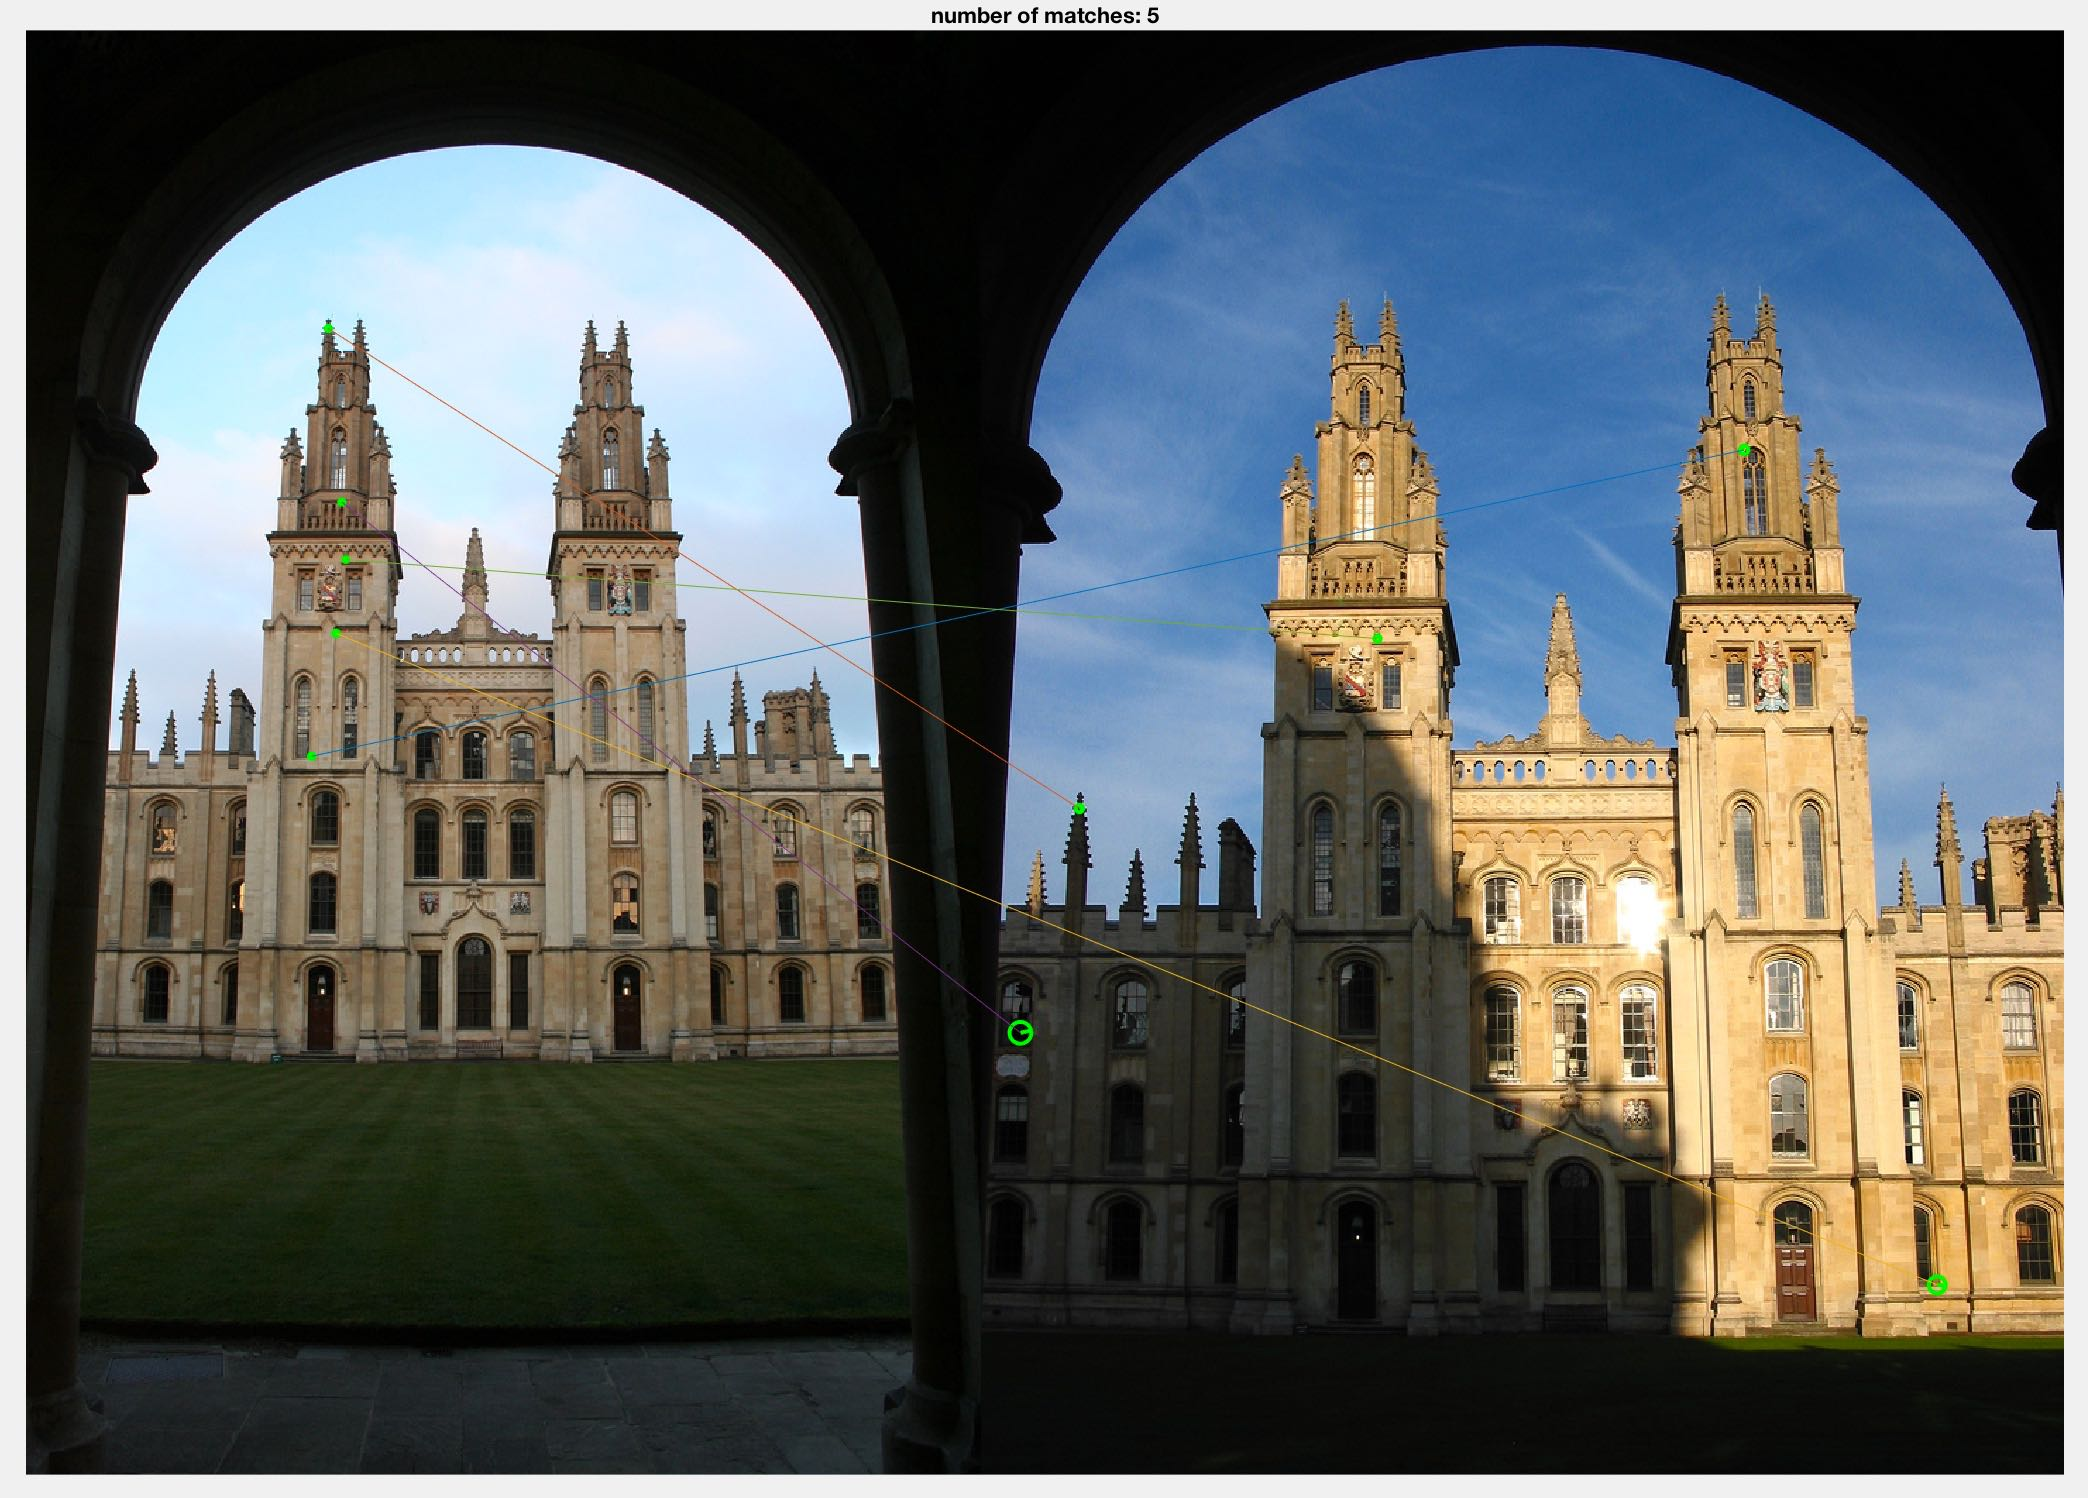
\includegraphics[width=15cm]{figure/mismatch.jpg}
\caption{Examples of mismatch with the simple nearest neighbors method}    
\label{mismatch_examples}
\end{figure}

Types of mistakes:
\\

- Recurrent patterns with different scale. The building on the images has some components that appear at several location with different scale. For instance windows or ornamentation (little peak on the roof) are appearing on each tower. Consequently it leads in some case to a mismatch as a peak on the left is matched to another peak on the right but not the same one. For instance on the figure \ref{mismatch_examples} it is showed by the red line, that match two different "peak" or the blue line that match two different window.

This effect is also amplified because the building is symmetric.
\\

- Big change in illumination. We saw that the change in lighting impact the density of feature detection in the darker area. Consequently all points with a match that are not in this dark area on the source image are obviously mismatched because they have no equivalent on the target image.\\


The current model miss some neighborhood features to decide among all possible matches in the target images which one is the right one that is relevant accord to the point in the source image. To remove mismatches, we could use the Lowe's second nearest neighbor test. This method forces the second nearest neighbor to be close to the first nearest neighbors, so that the match is not just a "co�ncidence", which give more robustness to the matching process.


\subsection{Improving SIFT matching (i) using Lowe's second nearest neighbor test}

\textbf{QIC.1: Illustrate and comment on improvements that you can achieve with this step. Include in your report figures showing the varying number of tentative matches when you change the nnThreshold parameter.\\}

\begin{figure}[!h]
\centering
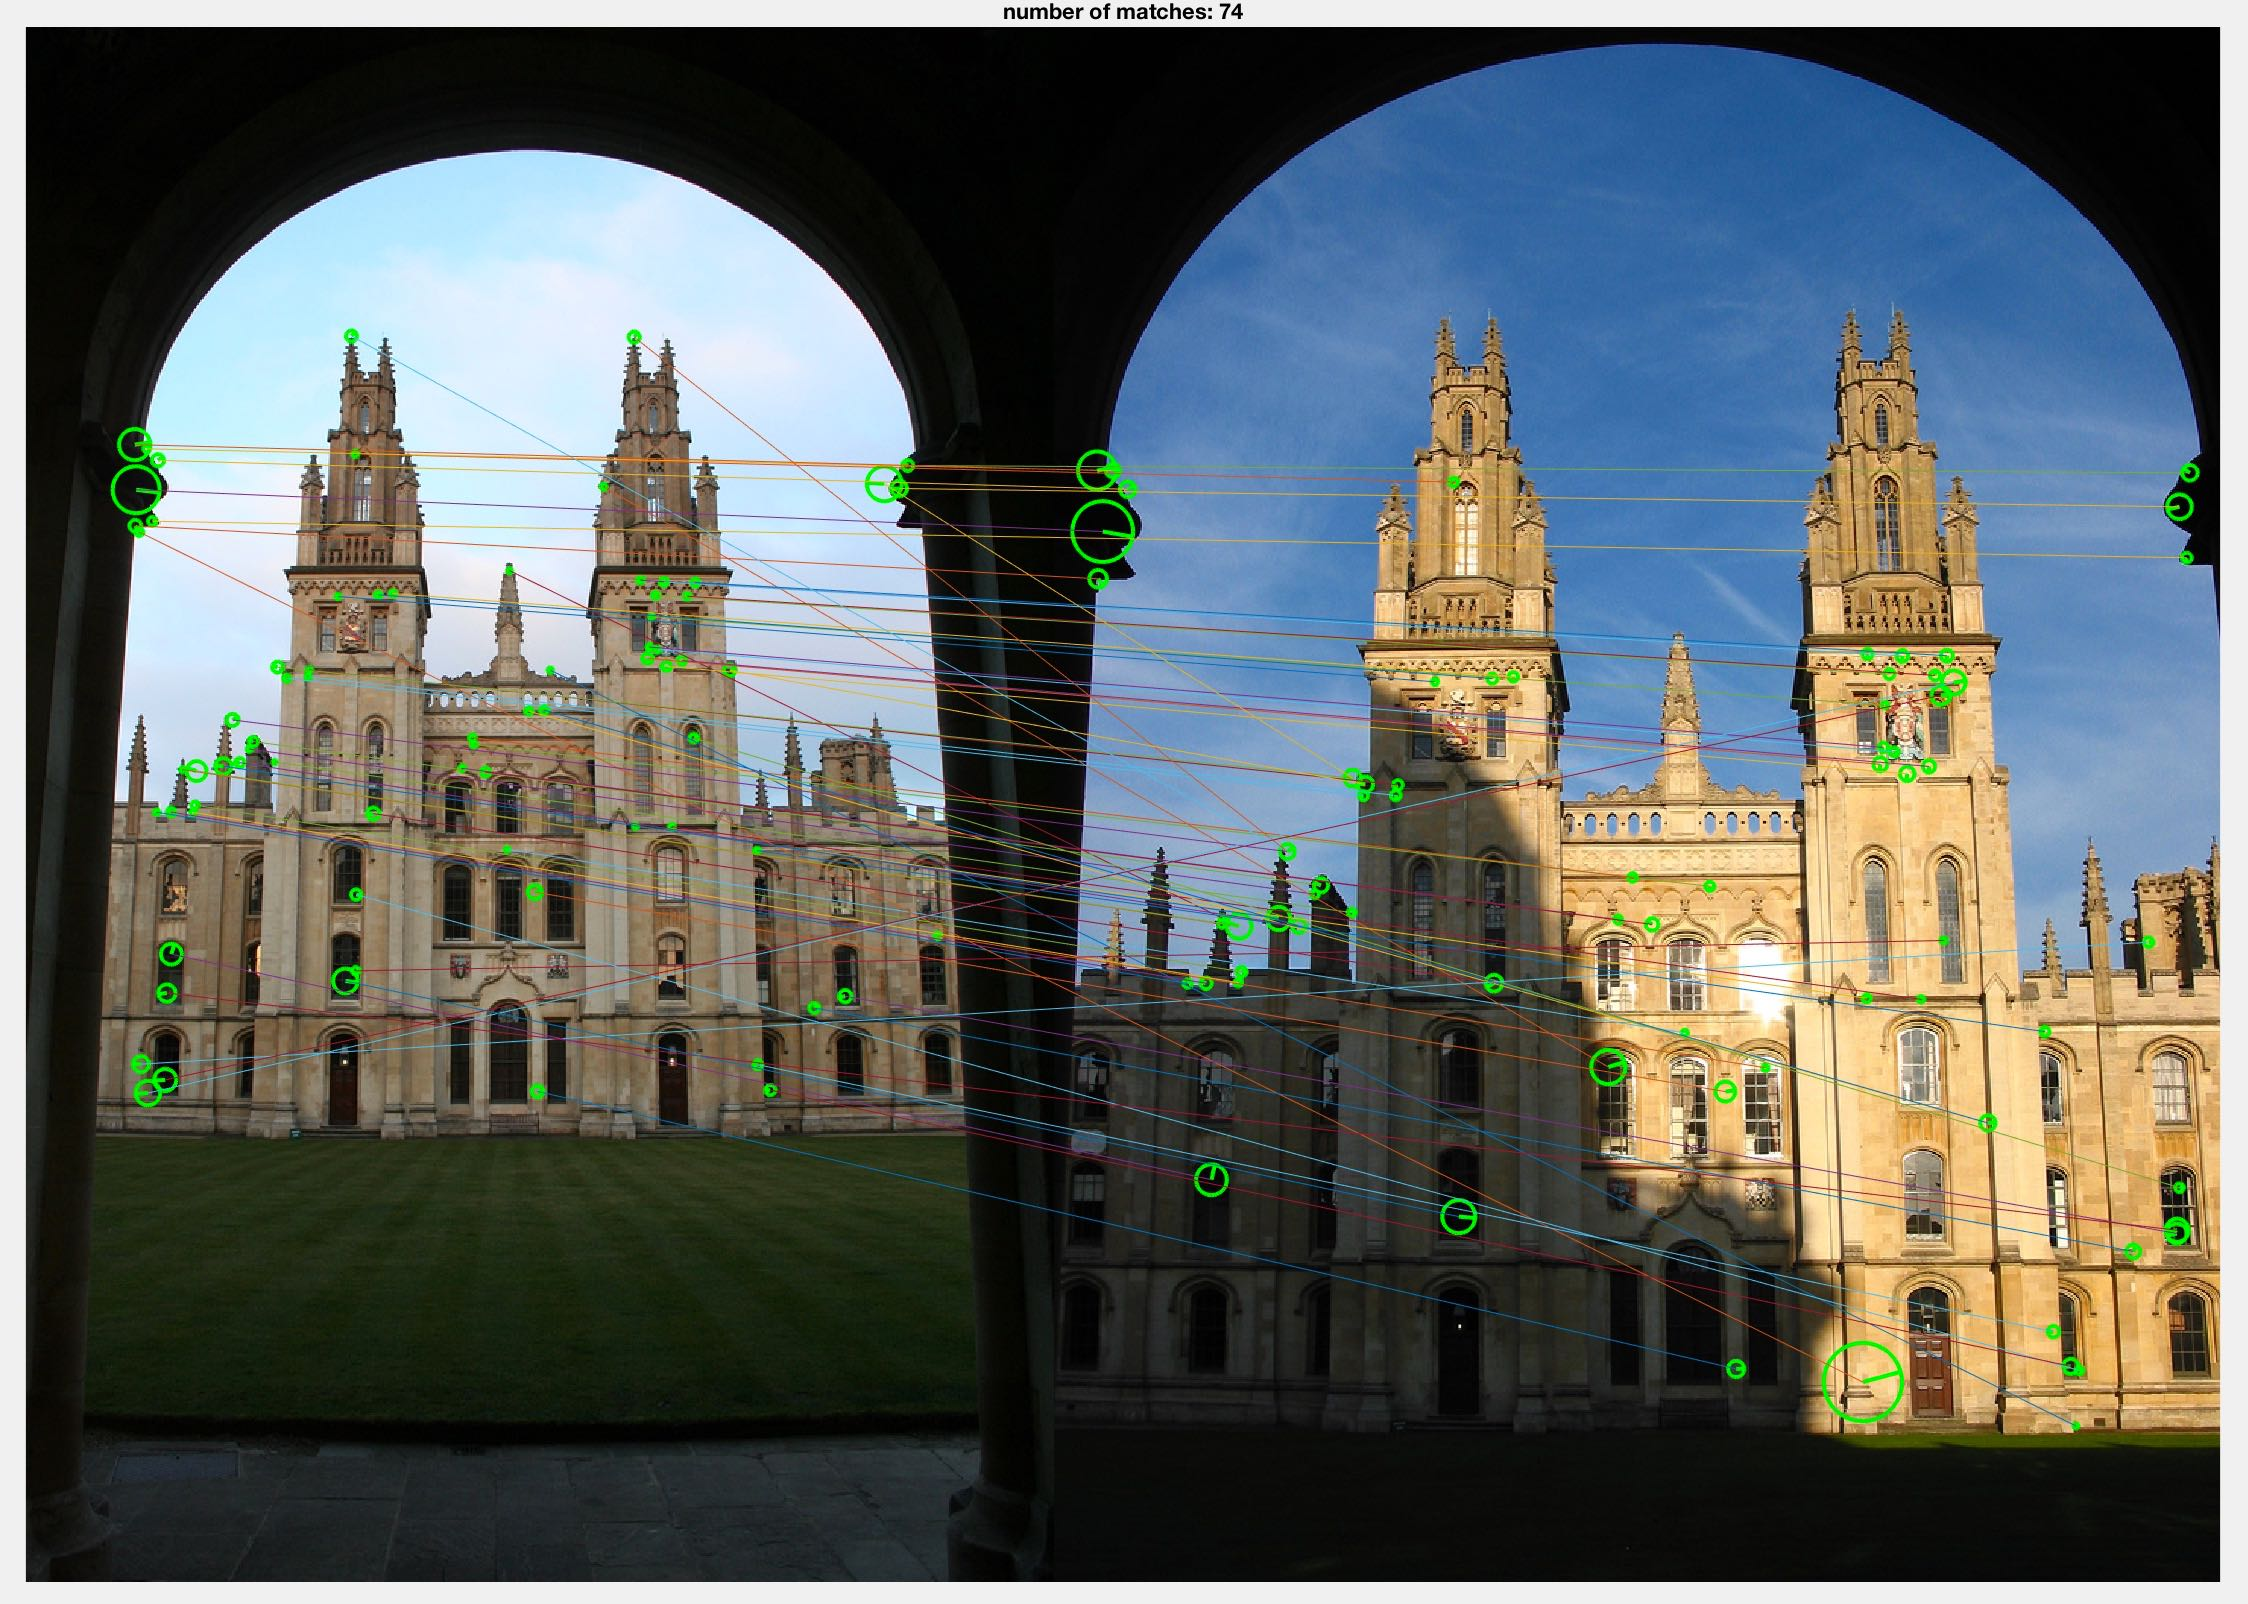
\includegraphics[width=13cm]{figure/matches_2nn.jpg}
\caption{Matches with the 2nd NN method}    
\label{matches_2nn}
\end{figure}

We use a value of 0.7 for nnThreshold for our comparaison. Which gives us about 150 matches. There is a real improvement in those matches. The figure \ref{matches_2nn} shows the new matches. Obviously we see that matches are much more accurate. However there are remaining issues with the points in the shadow that matches other point on the right images. Furthermore symmetry and recurrent patterns still make some mismatch.  \\

We tested the second nearest neighbor method for matching with different value of the nnThreshold in figure \ref{number_match}. Naturally the smaller the threshold is, the smaller the number of match is.

\begin{figure}[!h]
\centering
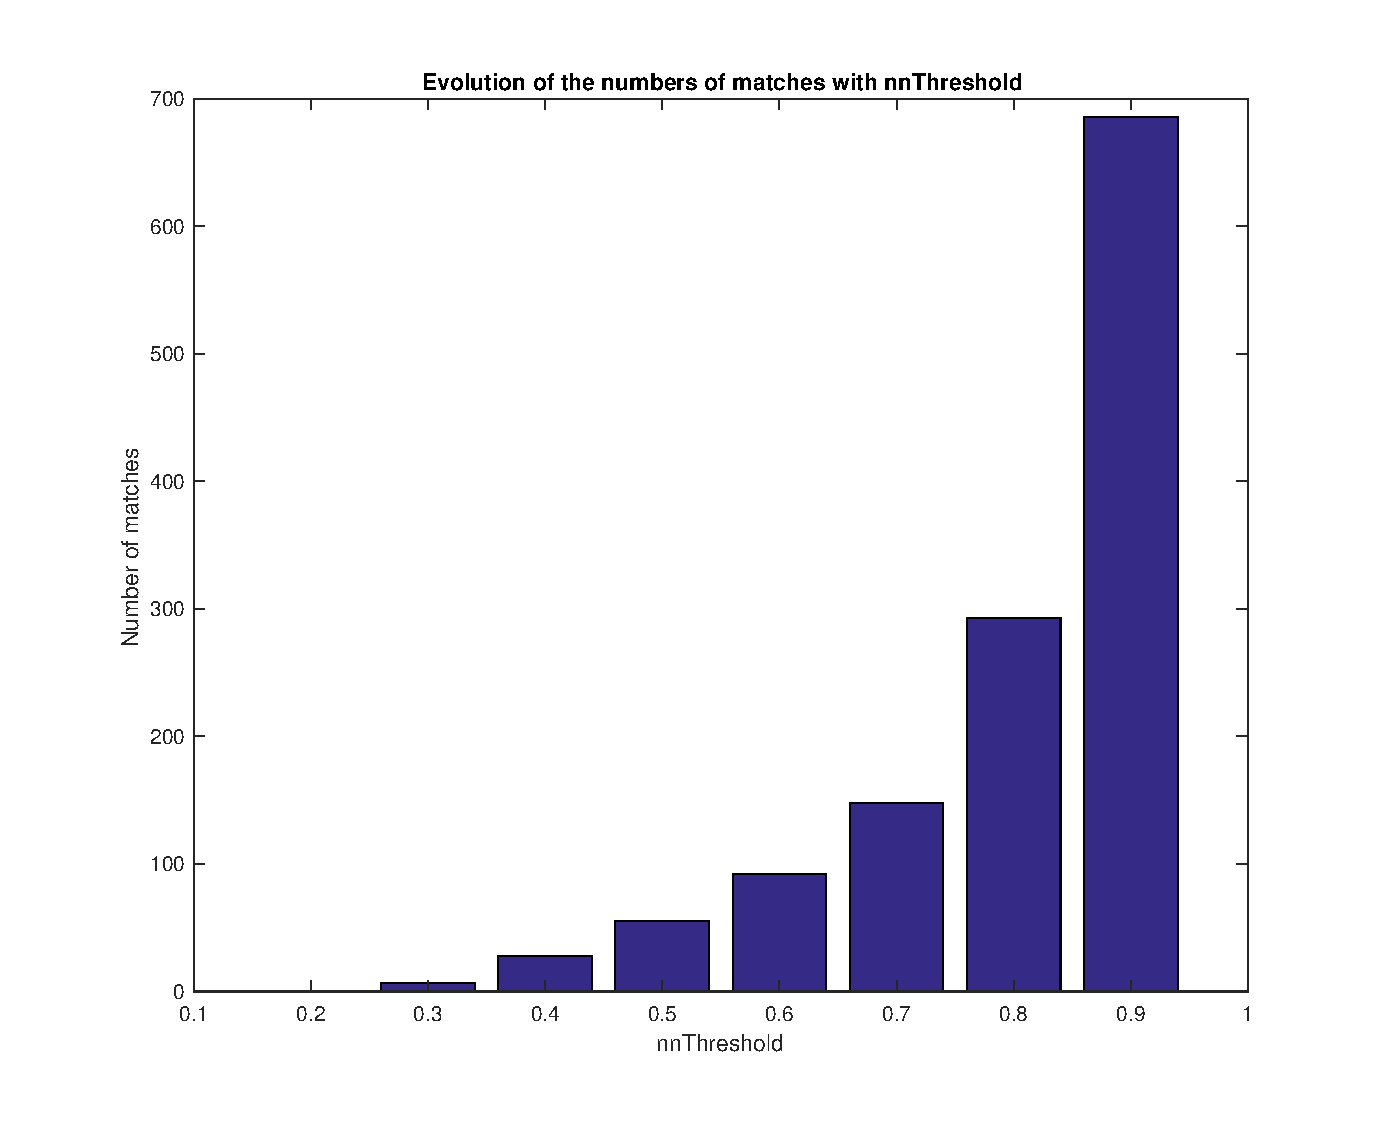
\includegraphics[width=13cm]{figure/number_match.eps}
\caption{Number of match with different value of nnThreshold}    
\label{number_match}
\end{figure}

\subsection{Improving SIFT matching (ii) using a geometric transformation}

\textbf{QID.1: Work out how to compute this transformation from a single correspondence.\\}

\textbf{QID.2: Illustrate improvements that you can achieve with this step.\\}

On figure \ref{match_compare_method}, we plotted the matches with each method we used in this assignment. We clearly see the steps of improvement looking at a bunch of match lines. Indeed the first simple method of NN produces many mismatch, we can see many lines that cross each other. The second one with the 2nd NN check allows to remove a bunch of mismatch but it remains some issues. The last method with Geometric Verifcation fixes all the remaining match issues (all lines are almost parallel).

\begin{figure}[!h]
\centering
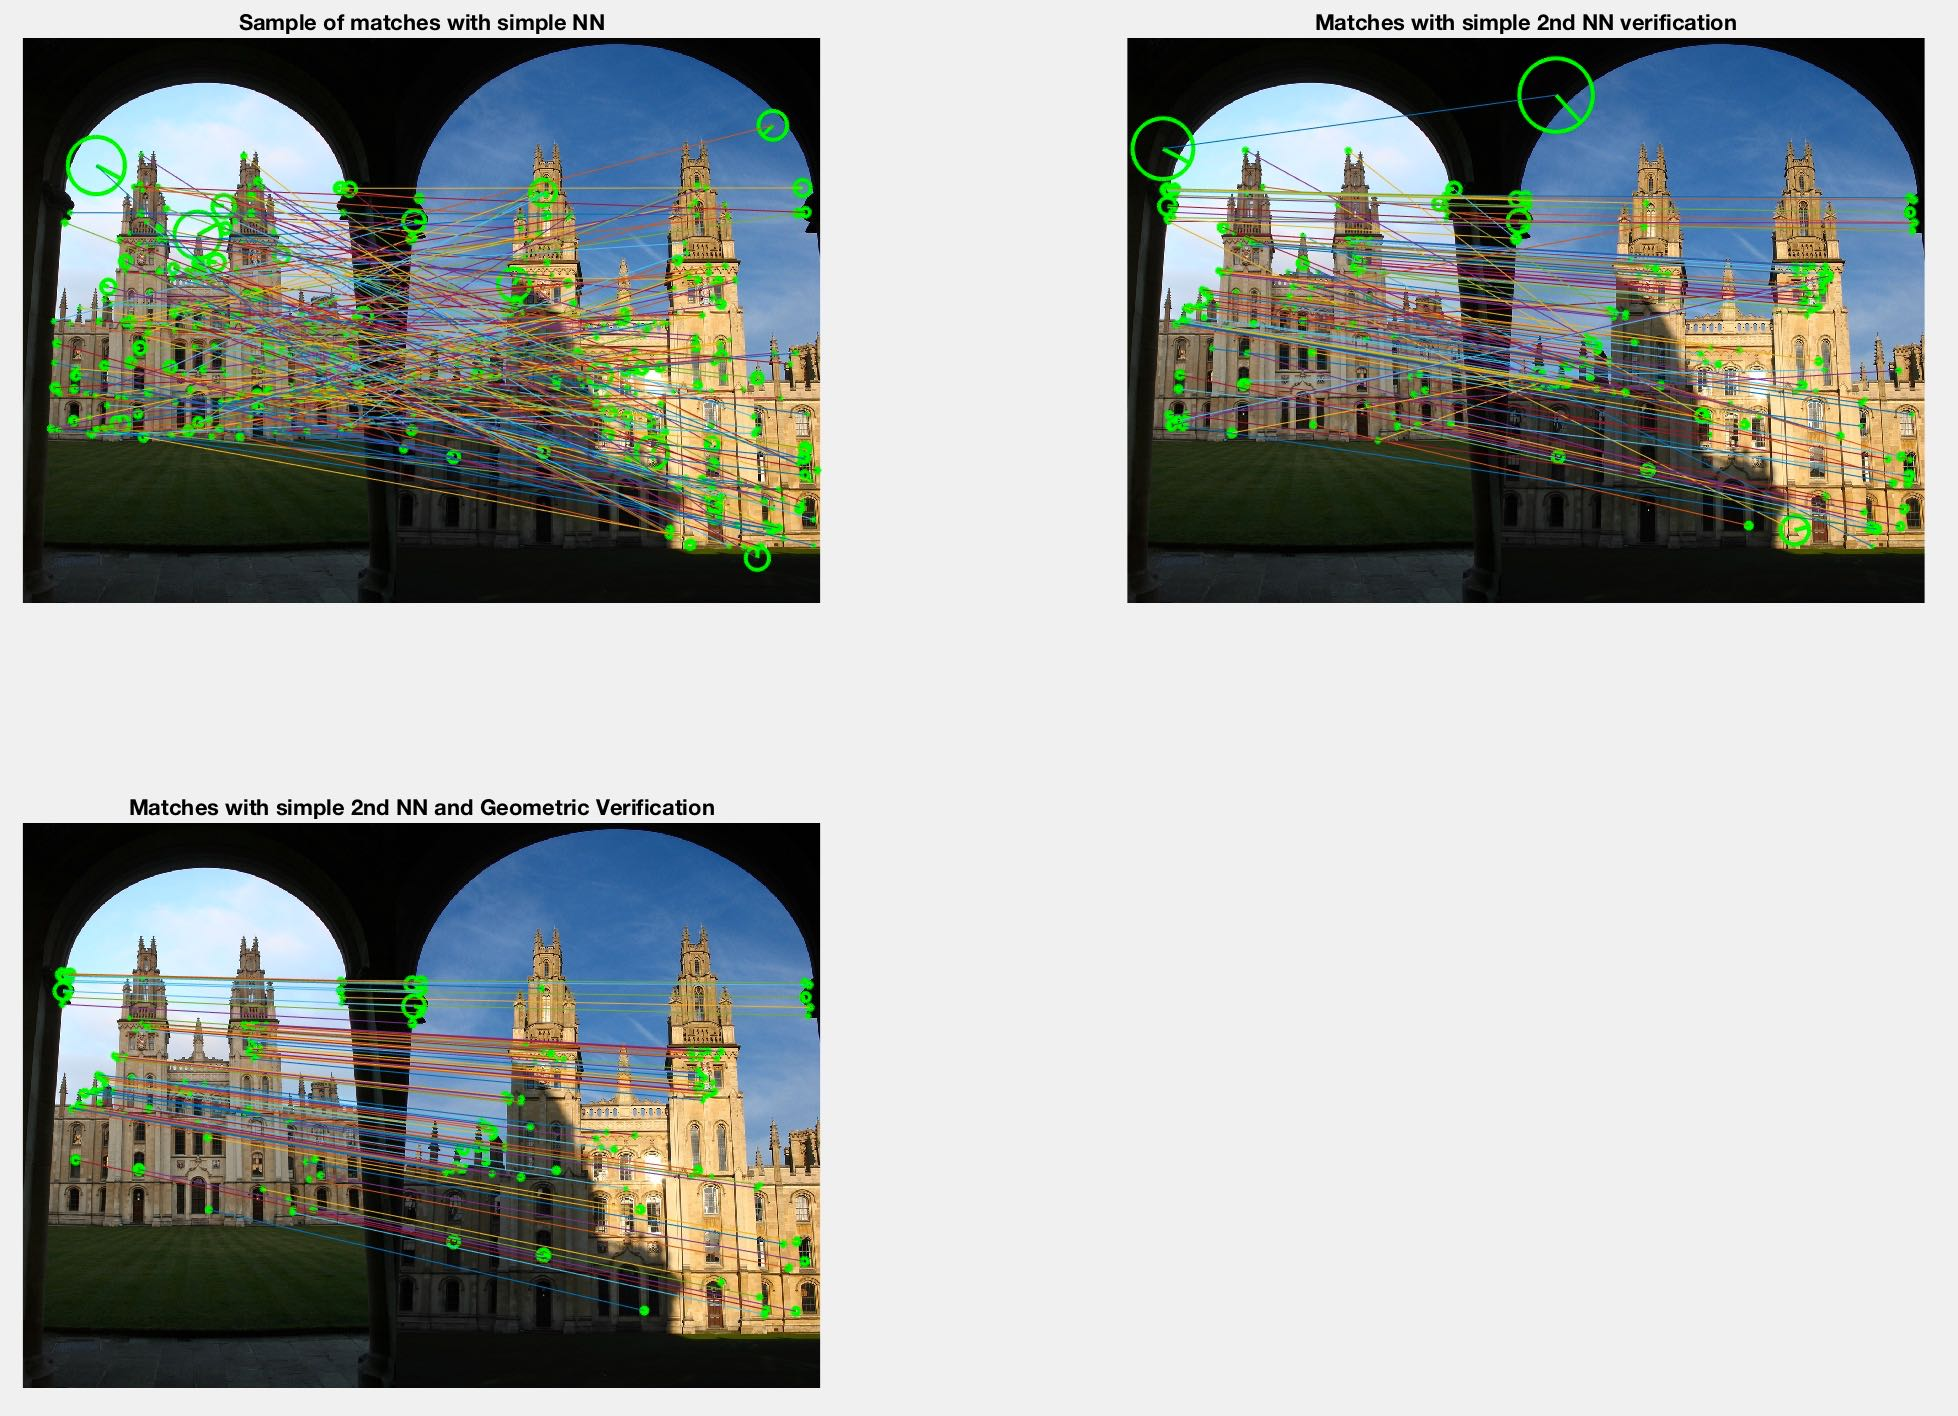
\includegraphics[width=15cm]{figure/match_compare_method.jpg}
\caption{Comparaison of each of method for the matching task. Top left: Simple NN, Top right: NN + 2nd NN check, Bottom left: NN + 2nd NN check + Geometric Verification}    
\label{match_compare_method}
\end{figure}

\clearpage

%----------------------------------------------------------------------------------------
%	Part II: Affine co-variant detectors
%----------------------------------------------------------------------------------------

\section{Affine co-variant detectors}

\begin{figure}[!h]
\centering
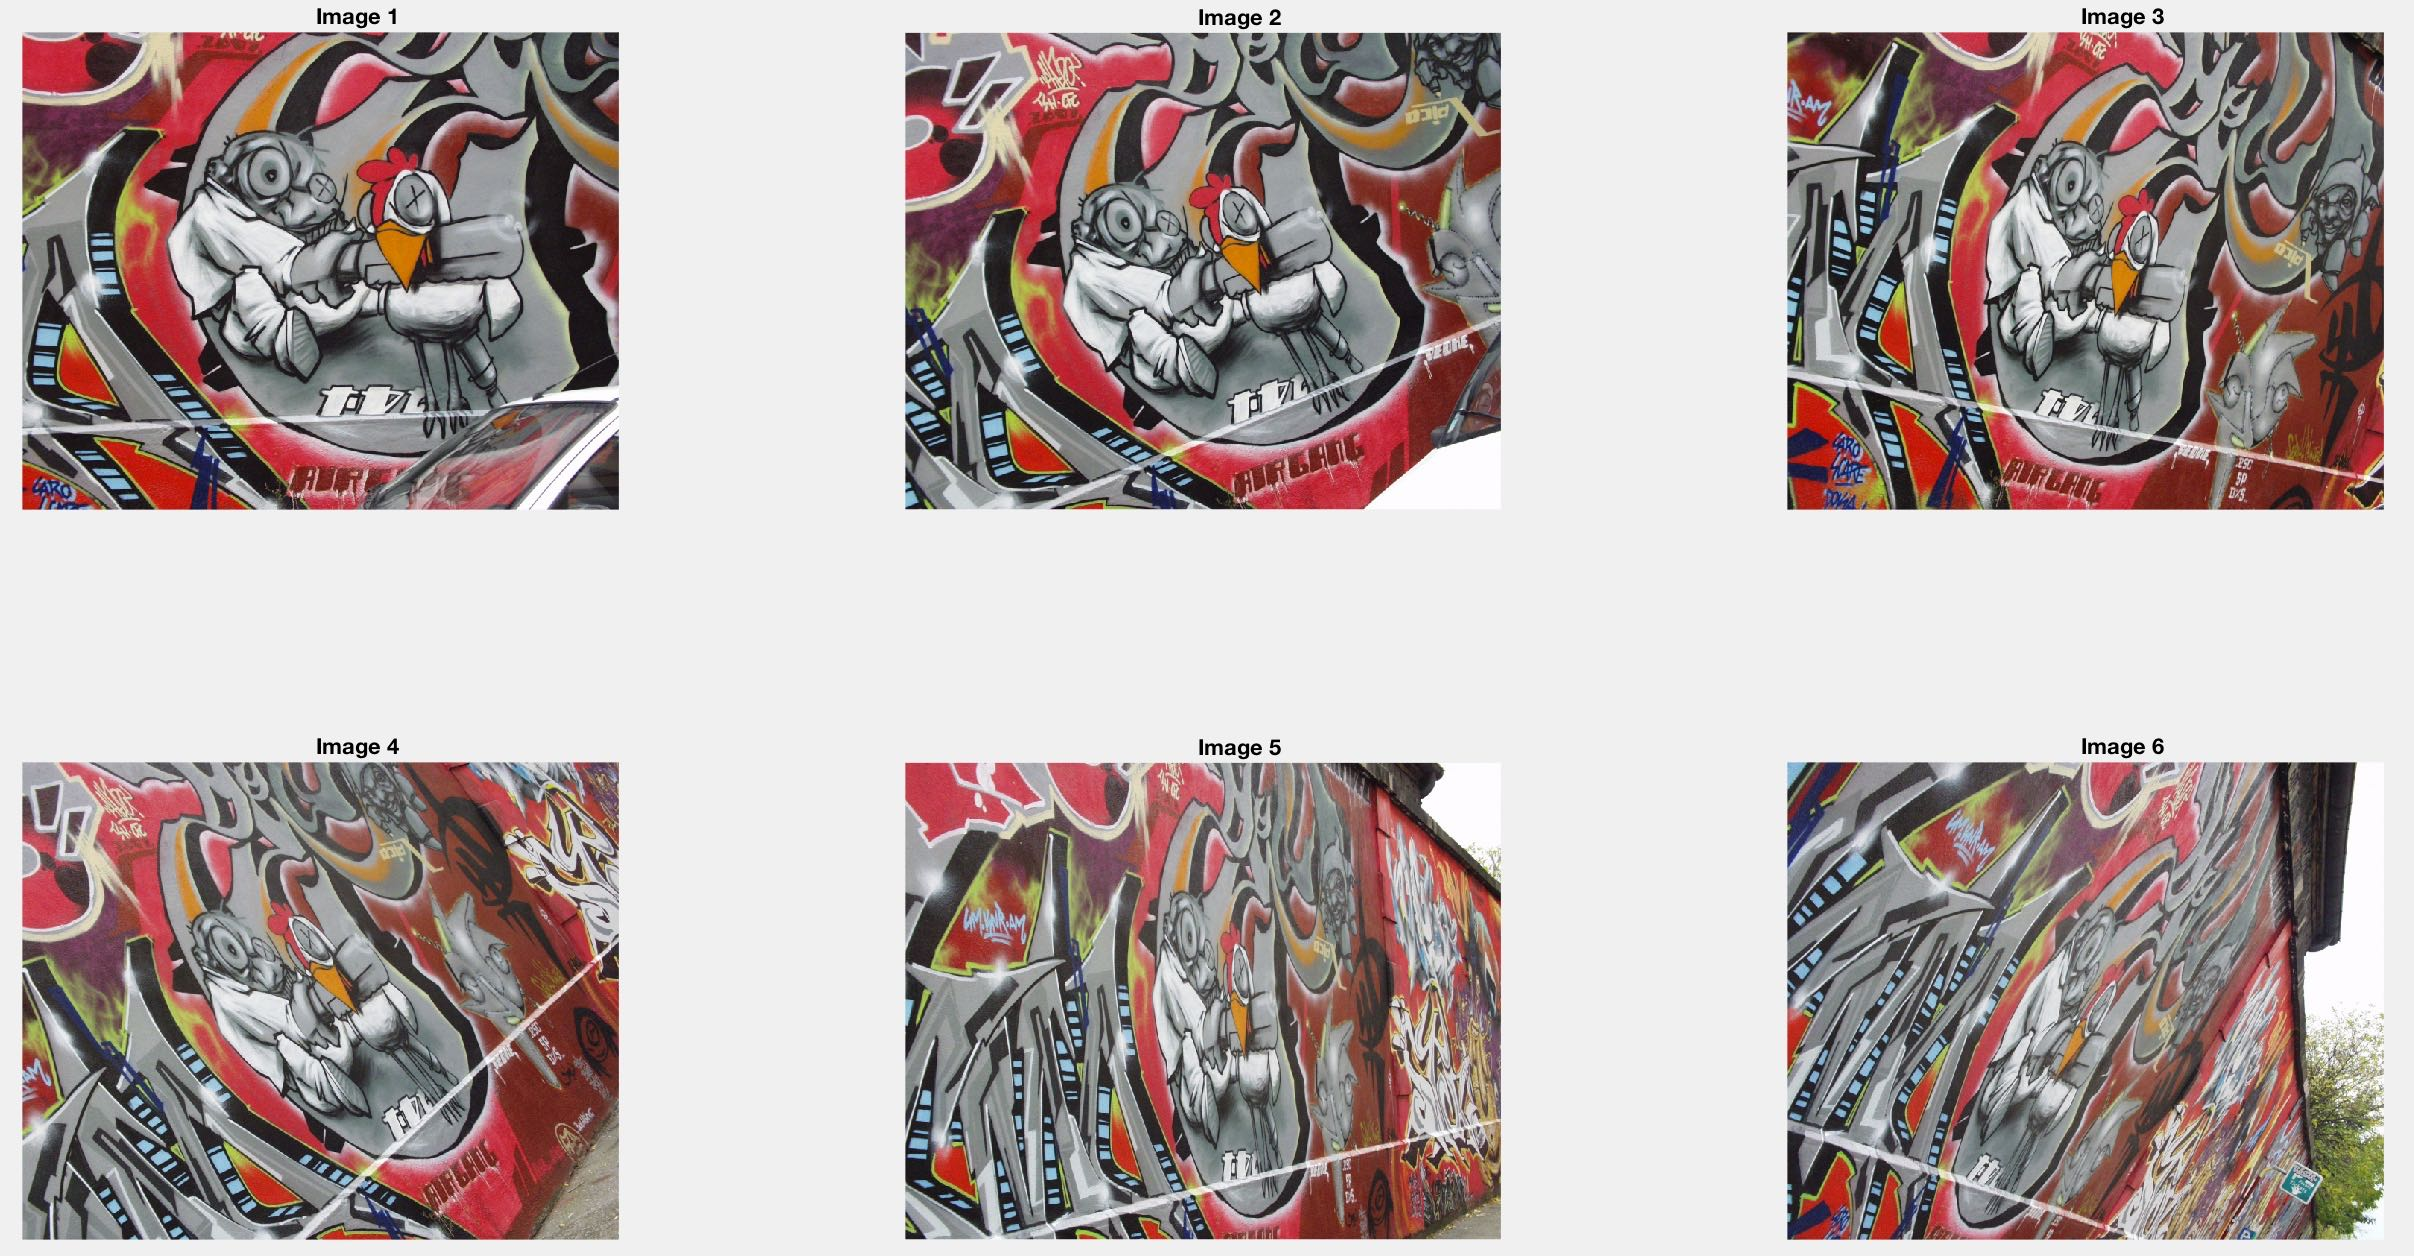
\includegraphics[width=18cm]{figure/images_part2.eps}
\caption{Plot of the 6 images used for this part II.}   
\label{images_part2}
\end{figure}

\textbf{QII.1: Show the number of verified matches with changing viewpoint. At first there are more similarity detector matches than affine. Why?\\}

In this part we try to match first image with each of the others images with index from 2 to 6. Each of theses pictures are represented in figure \ref{images_part2}. After executing the part-II script, we can compare the number of verified matches (after geometric verification) for each paire of images using two types of detectors : similarity detectors (SIFT detectors) and affine detectors (hessian-affine detectors). Results are plotted in Figure \ref{matches_number_similarity_affine}. \\

We observe that for the two paires (image1, image2) and (image1, image3) the similarity detectors provides more matches than the affine detectors. However starting from images 4 until the last one 6, we have better results with the affine detectors than the similarity one. \\

Why ? If we take a look at the raw images in figure \ref{images_part2}. We observe that images 2 and 3 are very different than images 4,5,6. Indeed images 2 and 3 could almost be simple rotation of image 1. However regarding images 4,5,6, there are much more perspective distortions. Consequently as similarity detectors are covariant with rotation (and translation) and do not try to find more complicated invariances it's quite normal that they perform well and even better than affine detectors on rotations of the first image. If affine detectors were "perfect" I guess they would perform equally with similarity detectors because similarity are part of affine transformation. But in practice, affine detectors try to find more complex transformation and consequently lose some performance on the first two images. However as soon as the change in view point increase affine detectors start to outperform similarity detectors as they succeed at finding the right anisotropic rescaling.

\begin{figure}[!h]
\centering
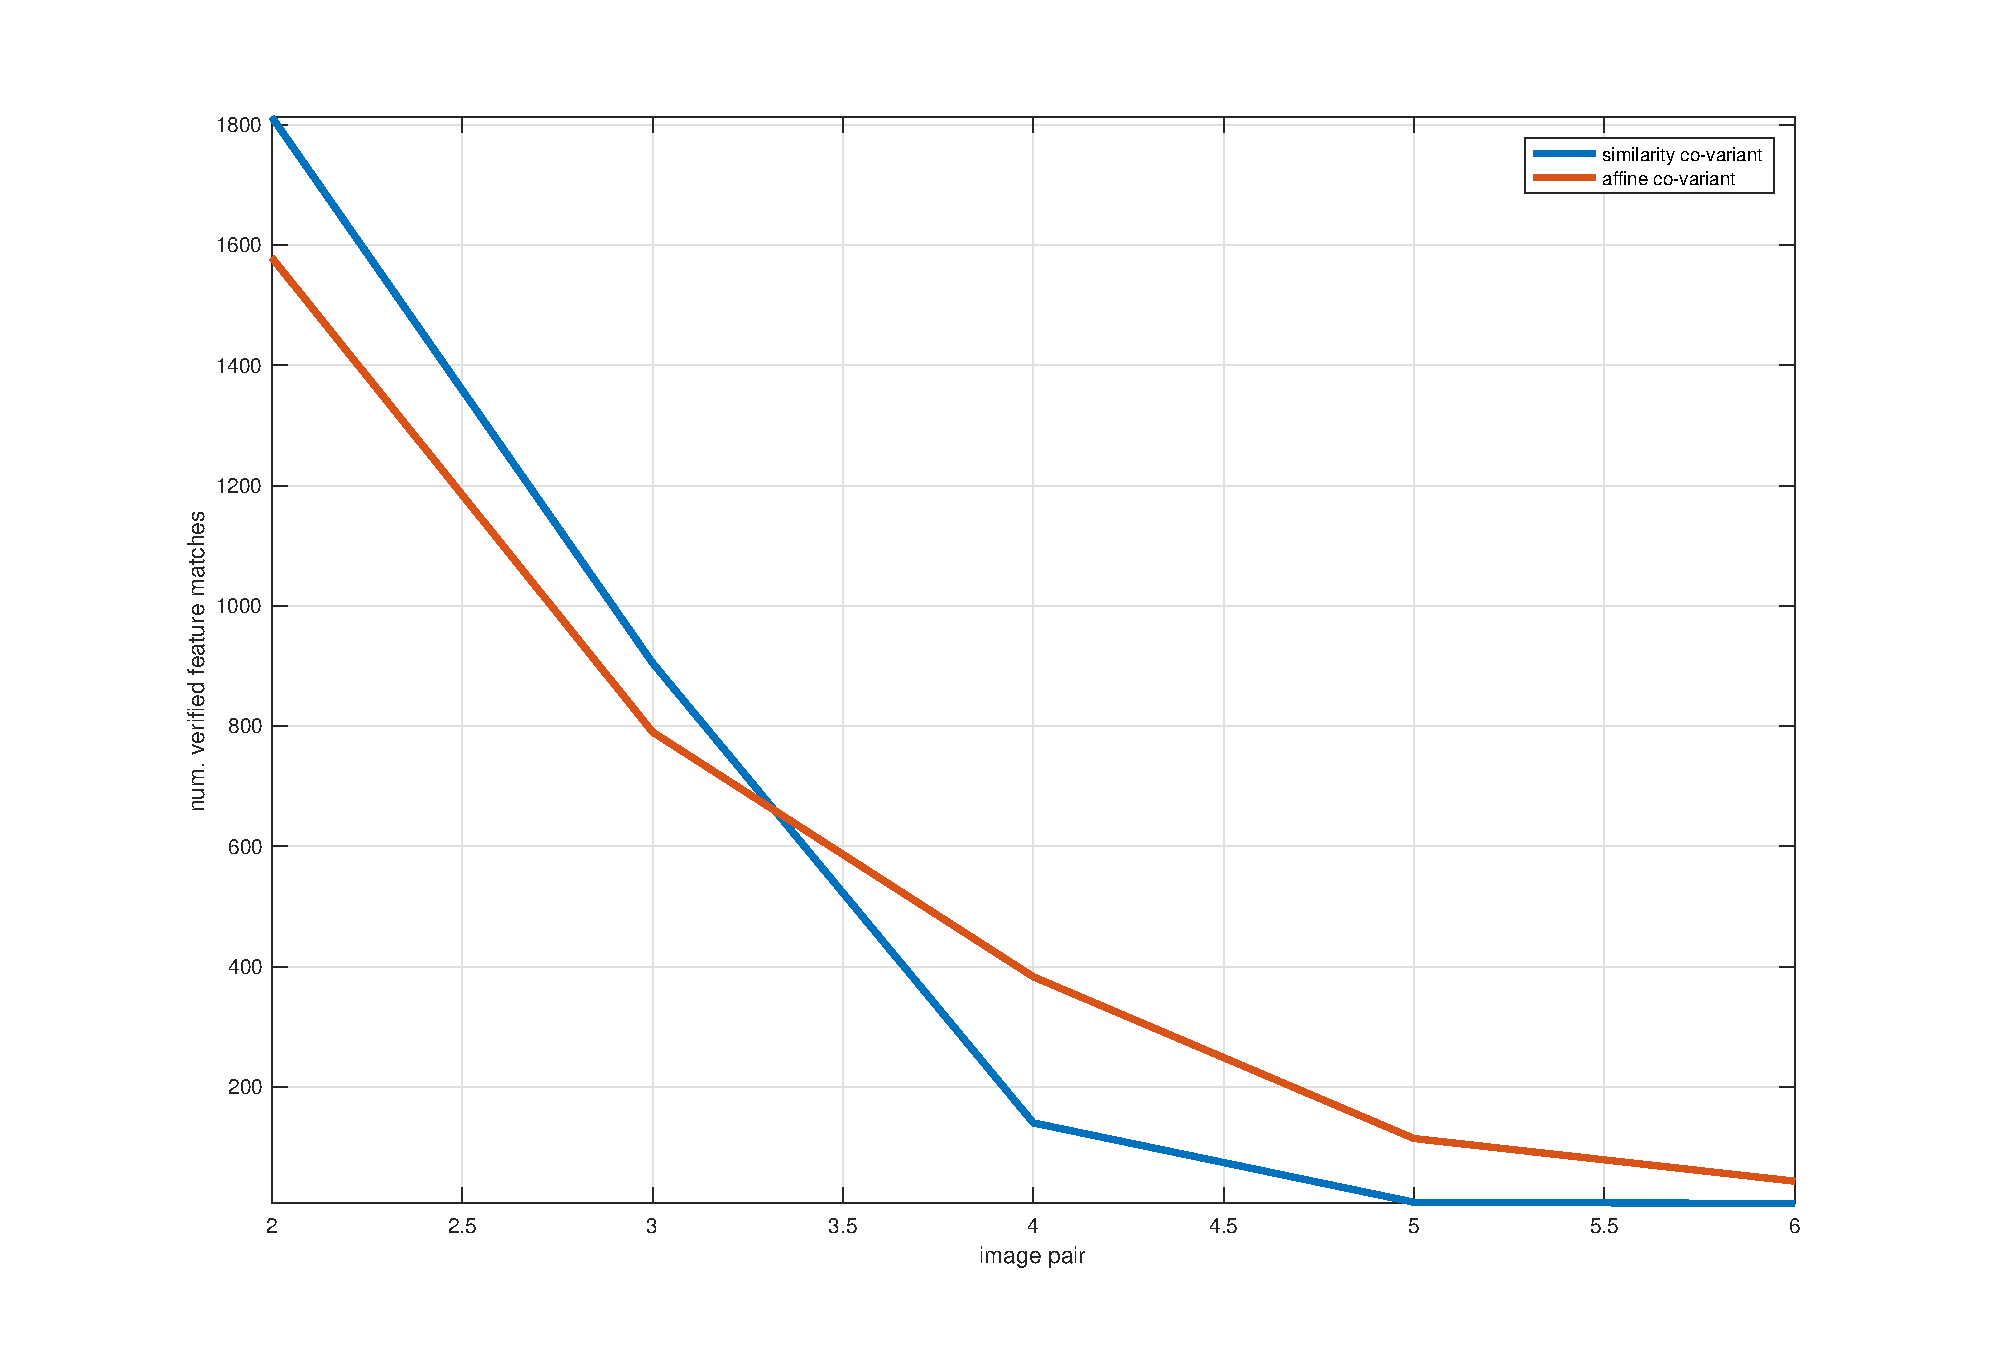
\includegraphics[width=13cm]{figure/matches_numbers_similarity_affine.eps}
\caption{Number of matches for paires (images 1, images k) for k = 2:6, with similarity detector in blue and affine detector in red.}   
\label{matches_number_similarity_affine}
\end{figure}

\clearpage

%----------------------------------------------------------------------------------------
%	Part III: Towards large scale retrieval
%----------------------------------------------------------------------------------------

\section{Towards large scale retrieval}

\subsection{Accelerating descriptor matching with visual words}

\textbf{QIIIA.1: In the above procedure the time required to convert the descriptors into visual words was not accounted for. Why the speed of this step is less important in practice?\\}

In the process of image matching for large scale retrieval, we have a query image and we want to find relevant matching images that are in our database. Consequently we want to index visual word vector of our images in DB instead of computing them on the fly because it's it more memory efficient than storing the whole descriptor for each image and it will be faster then as matchWords is just a scalar product (dot product). As a result the step where we compute visual words for the query image isn't significant compared to time it takes to compare each paires of visual word vectors.\\

\textbf{QIIIA.2: What is the speedup in searching a large, fixed database of 10, 100, 1000 images? Measure and report the speedup for 10, 100 and 1000 images.\\}

Using the im1 and im2, and comparing speed for getting the matches :

\begin{center}
	\begin{tabular}{ l | c  }
 		\hline			
   		Raw Descriptors & Quantized Descriptors \tabularnewline
  		\hline
    		0.1174s  & 0.0601s \tabularnewline
 		\hline  
 	\end{tabular}
\end{center}

We see that using the quantized descriptor is much faster. We then compare the efficiency for matching an image against a database of size varying from 10 to 300 images. We used the image database given in the data folder, which size is 660. Results are plotted on figure \ref{speed_comparison}.

\begin{figure}[!h]
\centering
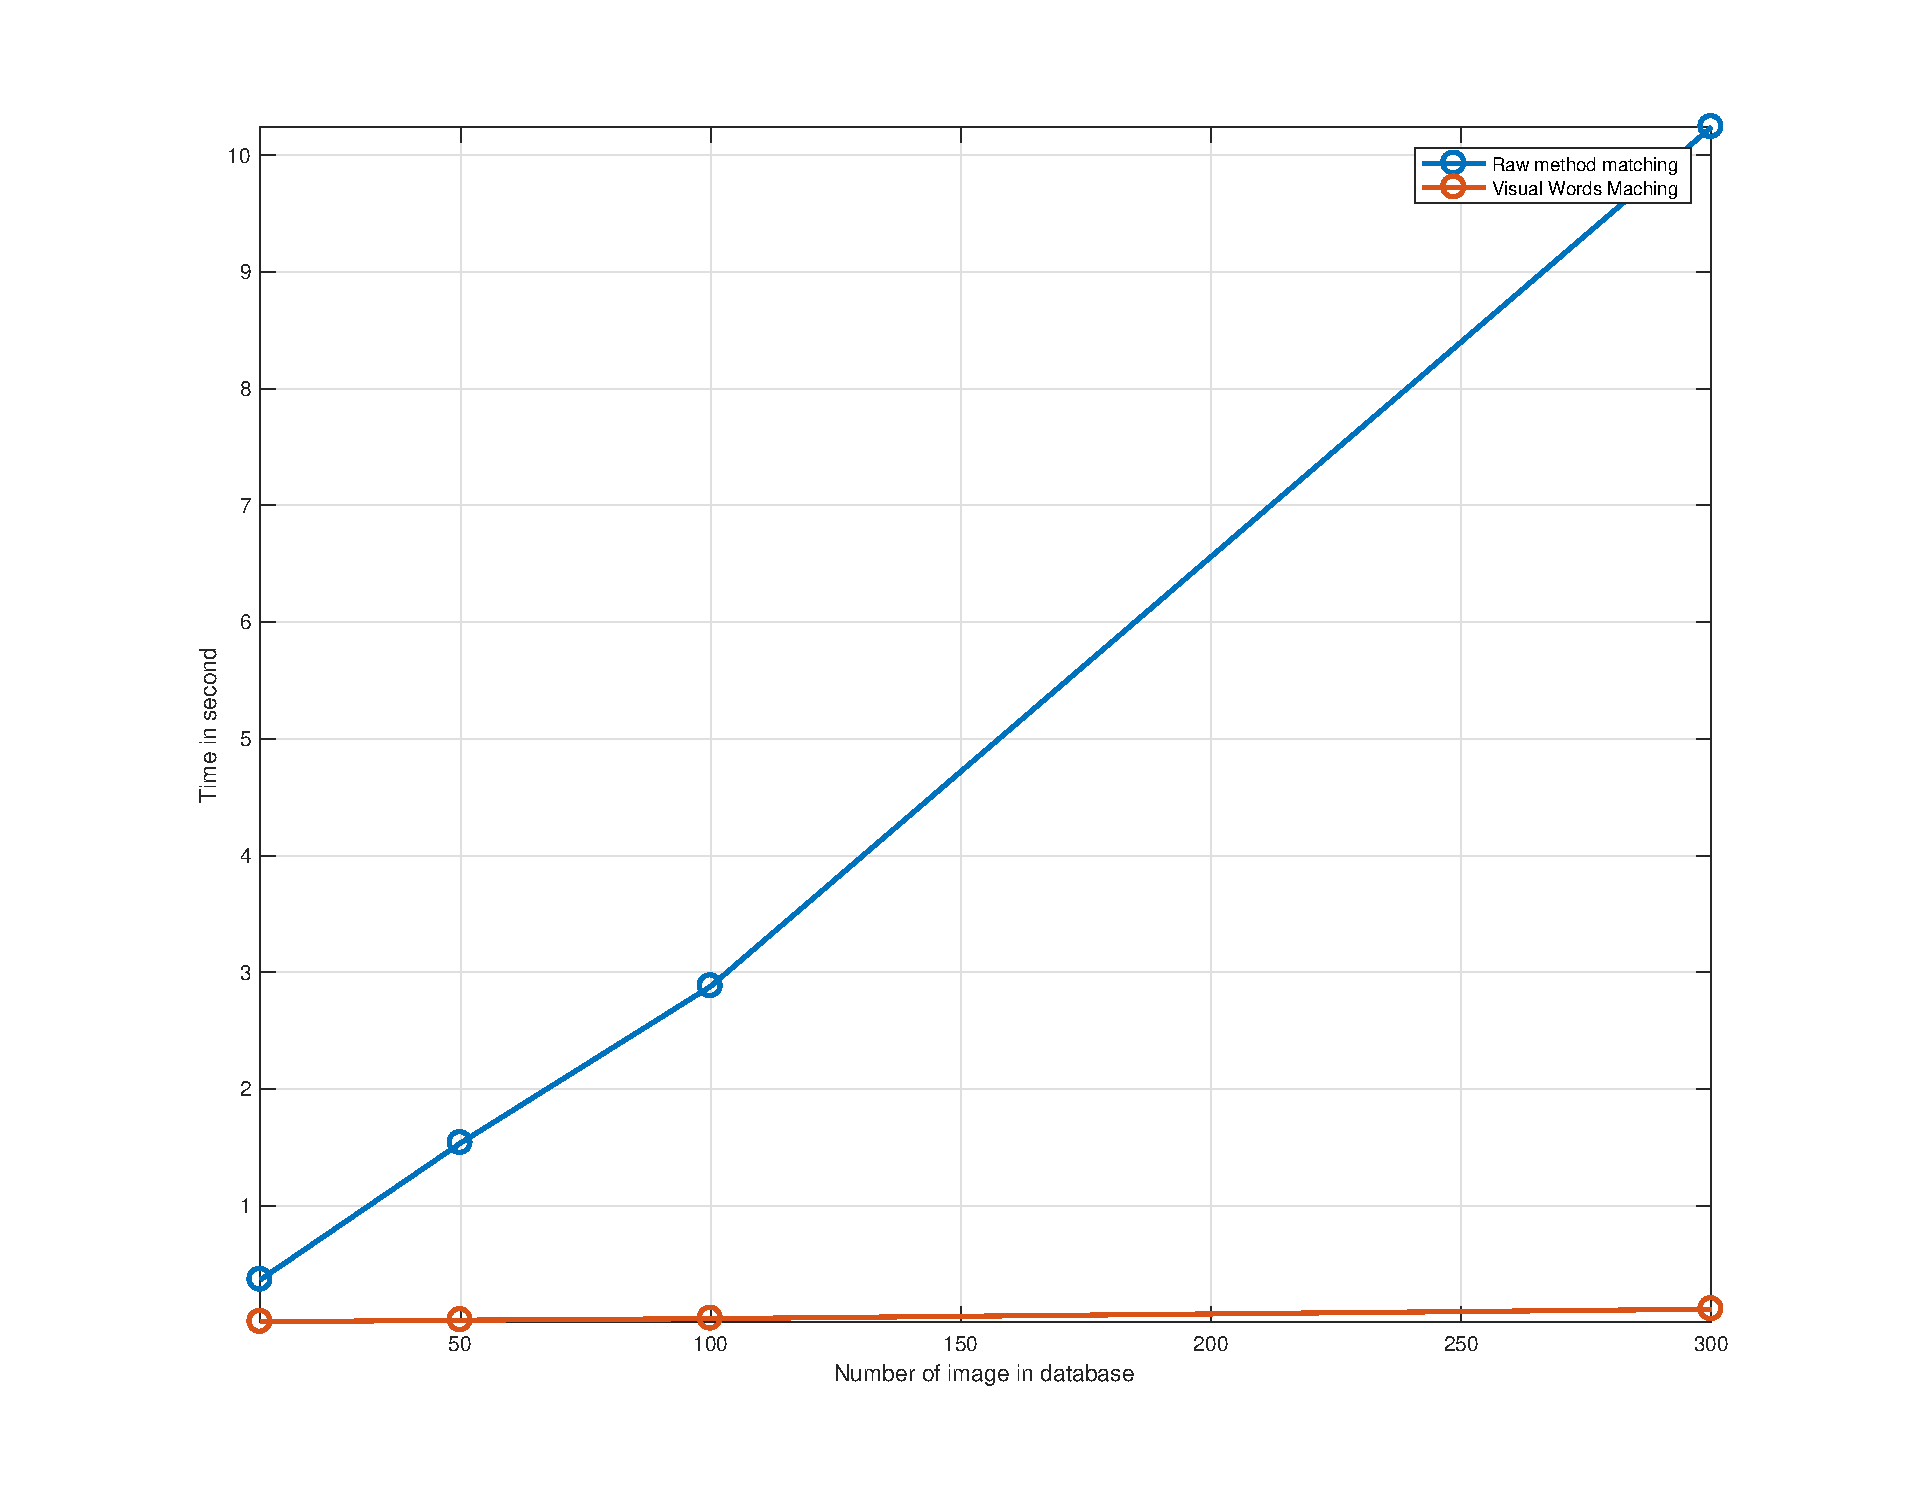
\includegraphics[width=11cm]{figure/speed_comparison.eps}
\caption{Matching speed comparison for different database size, using the raw descriptor in blue and the visual words in red.}   
\label{speed_comparison}
\end{figure}

We observe that using quantized descriptors dramatically decrease the time for processing all paires.\\


\textbf{Optional step\\}

We modified matchWords to generate more than one match for cases in which multiple features are mapped to the same visual word. Simply setting maxNumMatches to 2 for instance allows after geometric verification to increase the number of inliers to 44, which bring us to the same number of inliers as in the raw descriptors case. See figure \ref{optional} for the matches in the three cases. 

\begin{figure}[!h]
\centering
\includegraphics[width=15cm]{figure/optional.eps}
\caption{Matches with Raw descriptors on top left, Visual words on top right, and Visual words allowing more than one match on bottom left.}   
\label{optional}
\end{figure}

\subsection{Searching with an inverted index}

\textbf{QIIIB.1: Why does the top image have a score of 1?\\}

Here we are searching for similar images given a query "image 2". As this query image is also in the database, ('data/oxbuild\_lite/ashmolean\_000028.jpg'), among the result it should pop up as the first item, with a score of 1. Indent the inner product of this query image with itself give 1 because the vectors are l2-normalized.\\

\textbf{QIIIB.2: How many erroneously matched images do you count in the top results?\\}

The figure \ref{top_results} shows the 25 top results for the query image that is on the top left of the results. Among the 10 first results we count 3 wrong matches. Among the 25 results, there are 15 wrong matches.

\begin{figure}[!h]
\centering
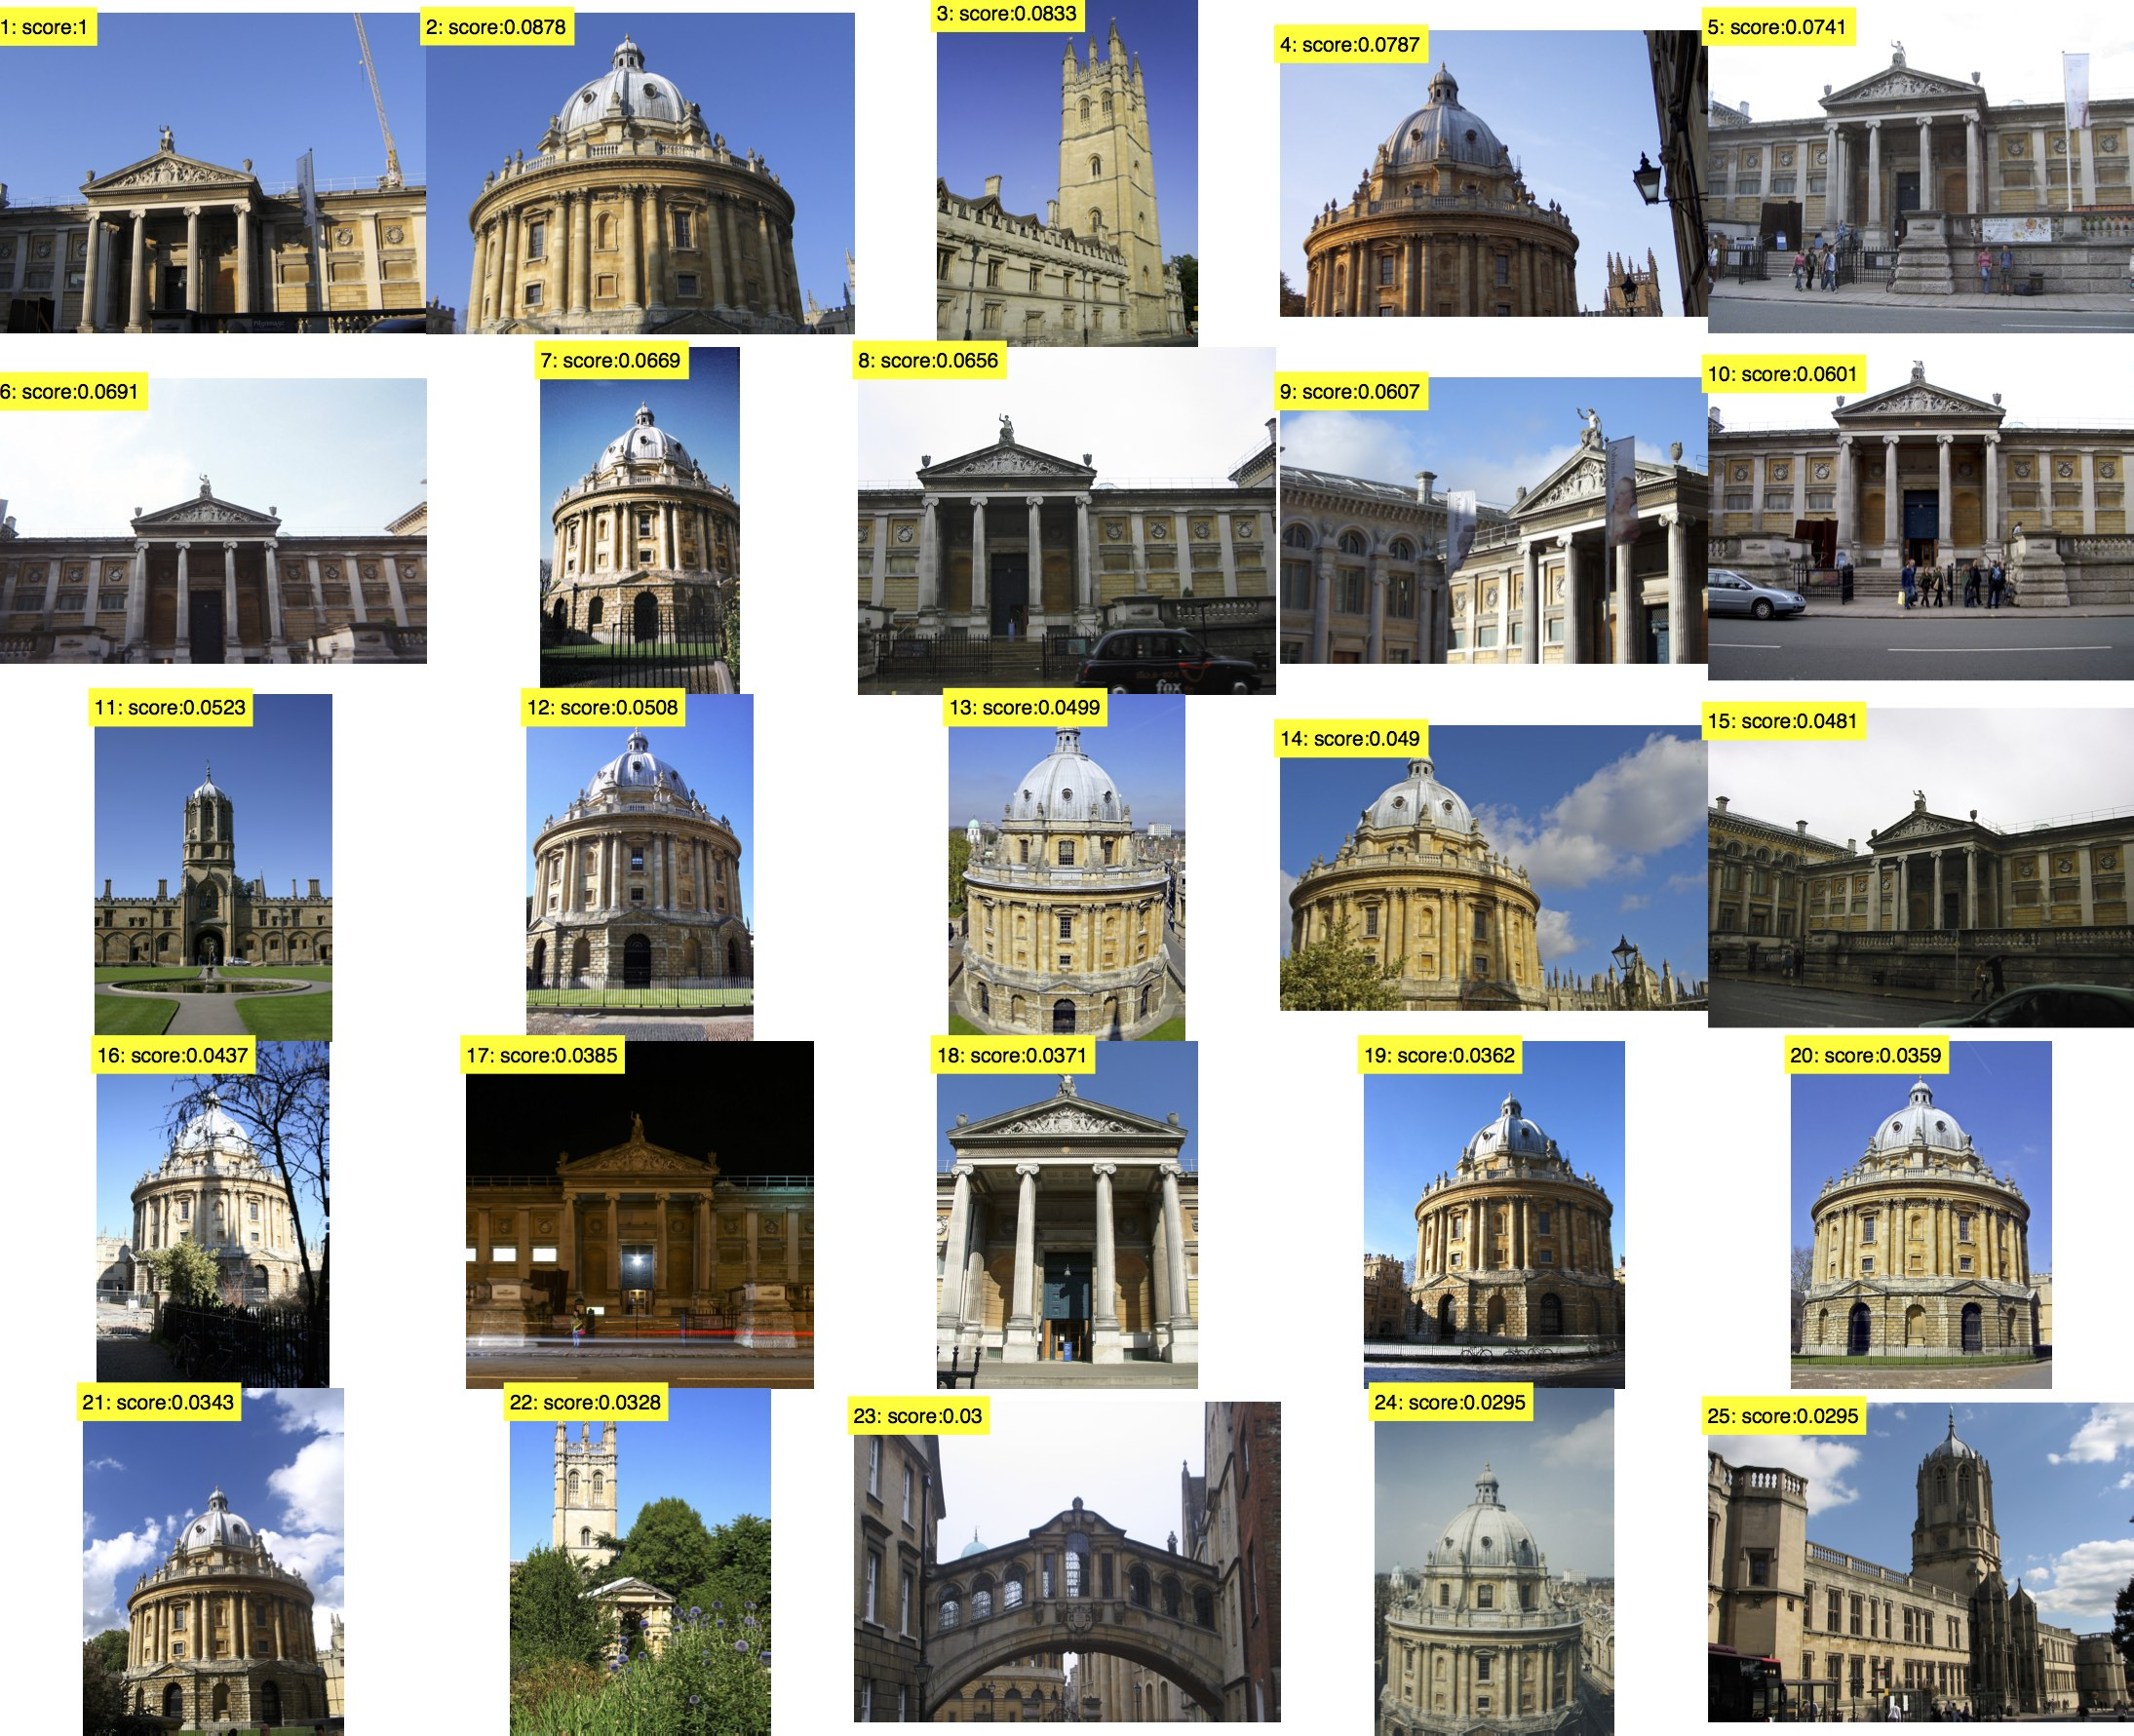
\includegraphics[width=12cm]{figure/top_results.jpg}
\caption{Top results for query image which is on the top left.}   
\label{top_results}
\end{figure}

\subsection{Geometric rescoring}

\textbf{QIIIC.1: Why is the top score much larger than 1 now?\\}

According to the re-ranking code :
\begin{lstlisting}
for rank = 1:25
  matches = matchWords(words,imdb.images.words{perm(rank)}) ;
  inliers = geometricVerification(frames,imdb.images.frames{perm(rank)},...
                                  matches,'numRefinementIterations', 3) ;
  newScore = numel(inliers) ;
  scores(perm(rank)) = max(scores(perm(rank)), newScore) ;
end
\end{lstlisting}

The new scores is the max between the number of inliers and the previous score. Consequently it's much larger than 1 for the top score, as indeed there are a lots of matches between the query image and itself. \\


\textbf{QIIIC.2: Illustrate improvements of retrieval results after geometric verification.\\}

Using the re-ranking after geometric verification give us many improvements. If we look at the top 10 results of the figure \ref{top_results_reranked}, we now have only 1 wrong match. Actually after the 9 first results, every following isn't related to the query image. Which mean that we retrieved all image that our database have that matches the query image. Following results are just similar buildings with similar architectures.

\begin{figure}[!h]
\centering
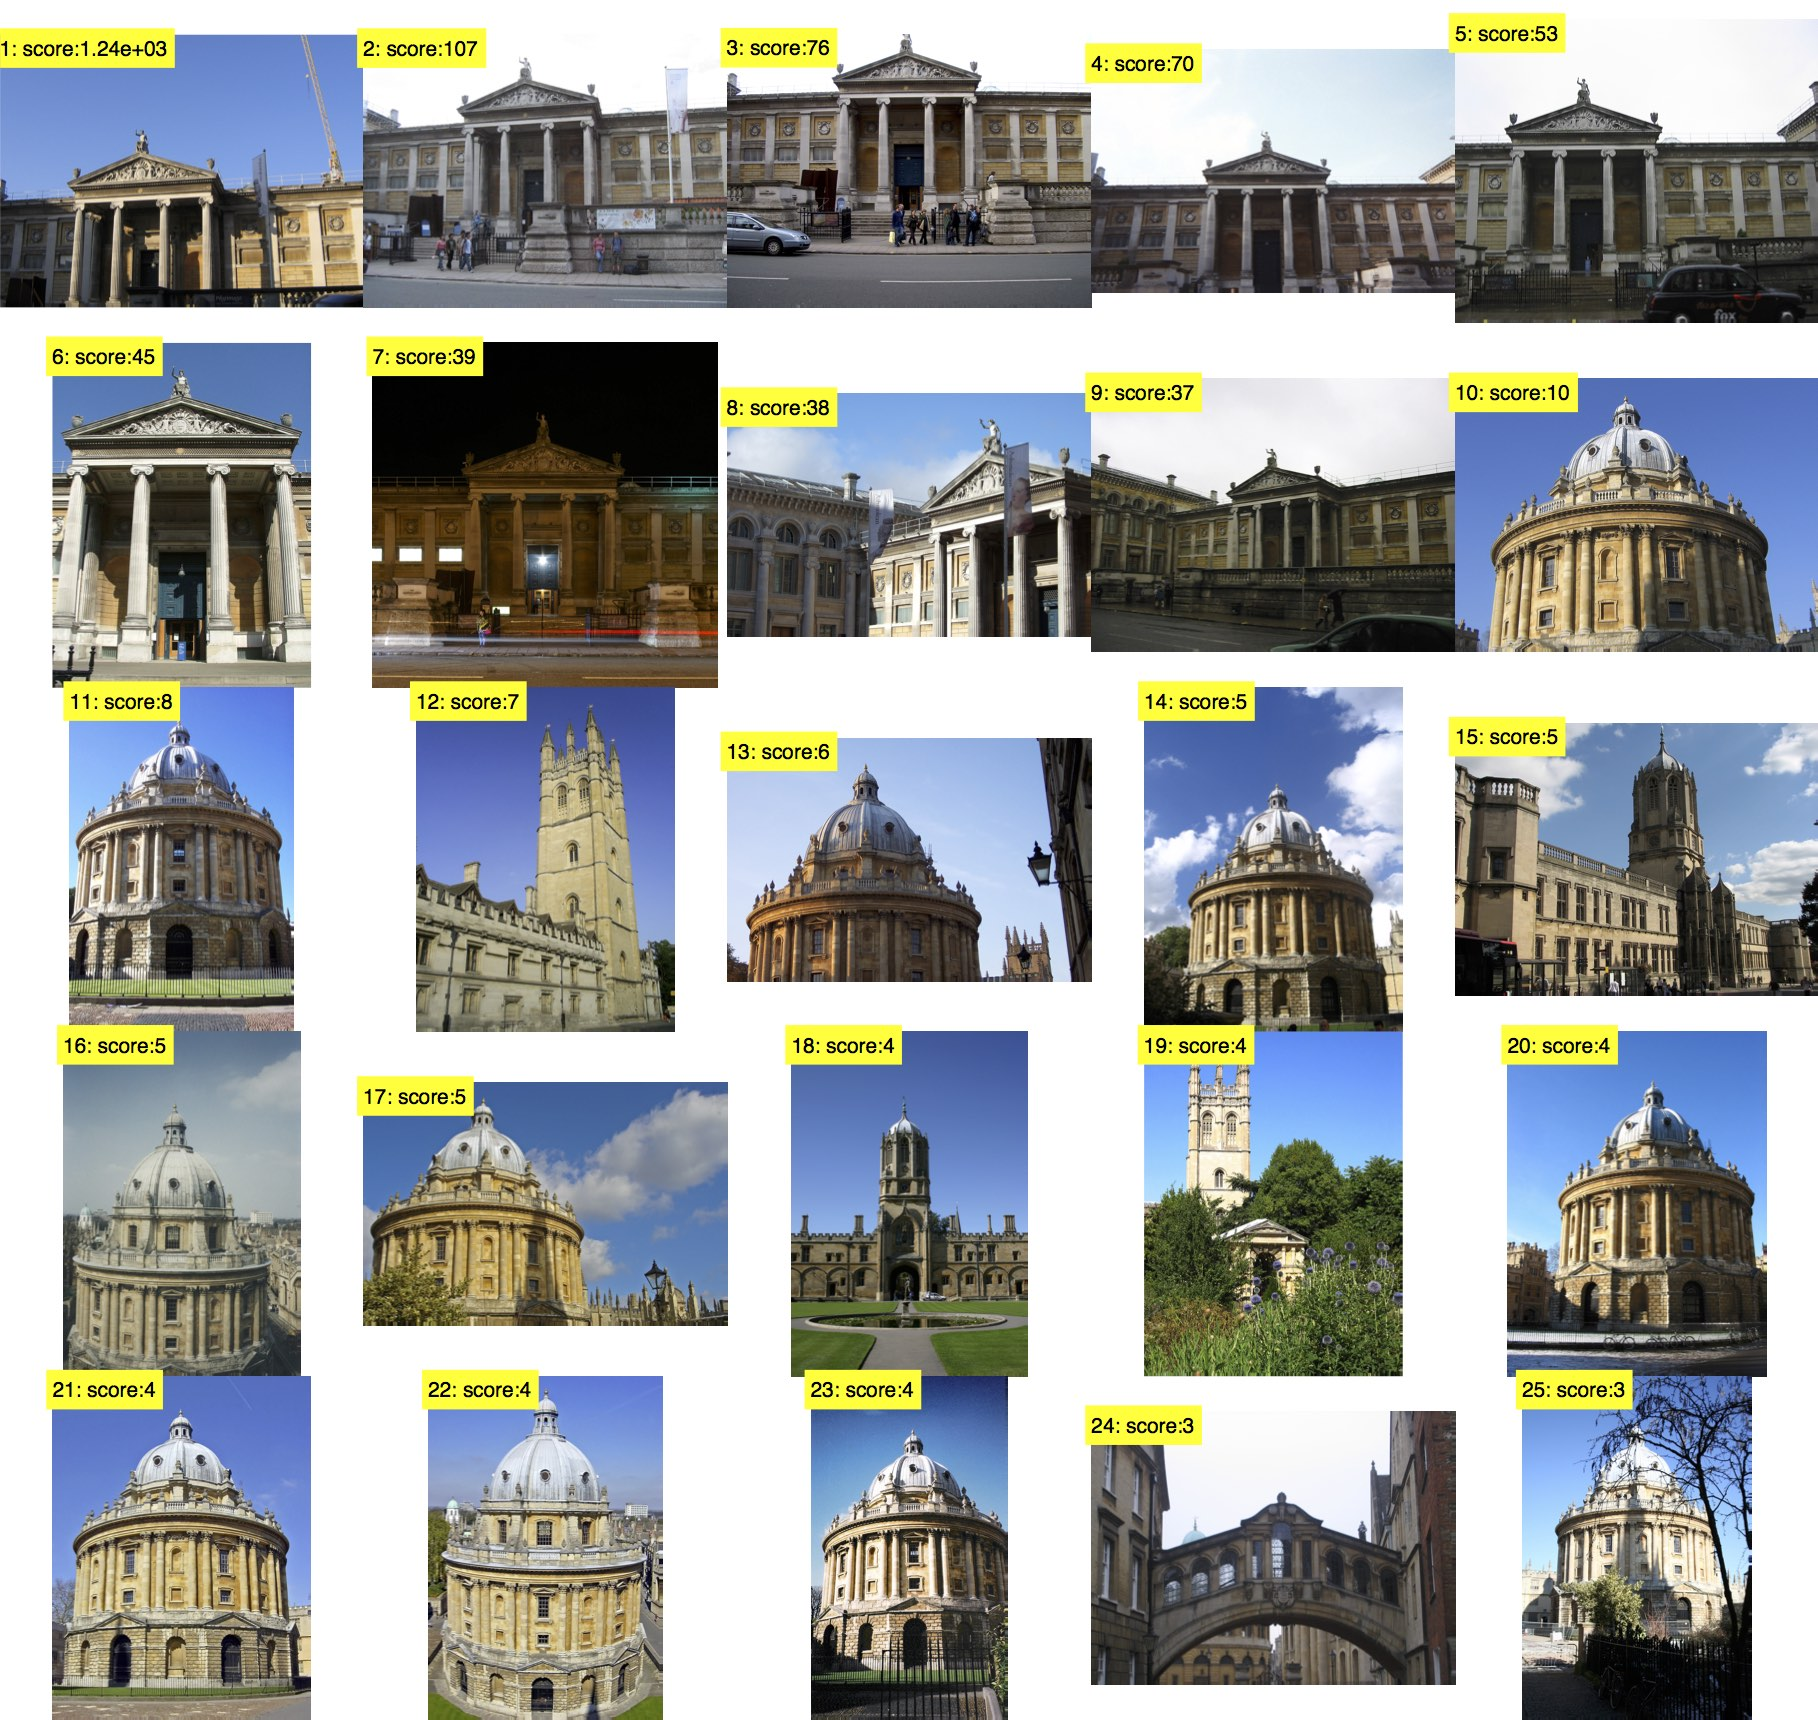
\includegraphics[width=12cm]{figure/top_results_reranked.jpg}
\caption{Top re-ranked results for query image which is on the top left.}   
\label{top_results_reranked}
\end{figure}

\clearpage

%----------------------------------------------------------------------------------------
%	Part IV: Large scale image retrieval
%----------------------------------------------------------------------------------------

\section{Large scale image retrieval}

\textbf{QIV.1: How many features are there in the painting database?\\}
\begin{center}
	\begin{tabular}{ l c }
    \hline	
    numWords: & 100000 \\
    vocab: & [128�100000 single] \\
    shortListSize: & 100 \\
    sqrtHistograms: & 1 \\
    index: & [100000�1734 double] \\
    idf: & [100000�1 double] \\
   \hline  	
 	\end{tabular}
\end{center}

The art painting image database have a vocabulary of 100 000 words.\\

\textbf{QIV.2: How much memory does the image database take?\\}

Asking "whos imdb" to matlab returns :
\begin{center}
	\begin{tabular}{ c c c c }
   		 \hline	
   		  Name & Size & Bytes & Class \\
  		  imdb & 1x1 & 349989427 & struct \\ 
		\hline  	
 	\end{tabular}
\end{center}

The Image database takes about 350MB in memory.\\


\textbf{QIV.3: What are the stages of the search? And how long does each of the stages take for one of the query images?\\}

The search process follow the following steps:

\begin{enumerate}
	\item Build feature for the query images.
	\begin{enumerate}
		\item Compute SIFT features for the query images
		\item Quantise the descritpors of the query image to retrieve its visual words features.
	\end{enumerate}
	\item Find the most similar in the inverted index.
	\item Perform geometric validation to re-rank the results. (get matches between most similar paires + geometric verification)
\end{enumerate}

For each images, the following table shows time spent per steps.

\begin{center}
	\begin{tabular}{ c |  c c c }
   		 \hline
		   & url1 & url2 & url3 \\	
		   \hline
   		  feature time &  0.339 s & 0.540 s &  1.914 s \\
  		  index time & 0.022 s & 0.025 s & 0.030 s \\
		  geometric verification & 0.392 s &  0.652 s & 2.220 s \\
		\hline
 	\end{tabular}
\end{center}

We finally see that expensive steps are features building: SIFT and then the geometric verifcation at the end. But the "index" step which look for similar images in the index is very efficient.

\begin{figure}[!h]
	\centering
	\includegraphics[width=13cm]{figure/vangoghresult.eps}
	\caption{Top result for mistery image 2: Wheat Field with Cypresses of Vincent van Gogh}   
	\label{vangoghresult}
\end{figure}


%----------------------------------------------------------------------------------------
%	BIBLIOGRAPHY
%----------------------------------------------------------------------------------------

\bibliographystyle{apalike}

\bibliography{sample}

%----------------------------------------------------------------------------------------


\end{document}